\documentclass[paper=letter,11pt]{scrartcl}

\KOMAoptions{headinclude=true, footinclude=false}
\KOMAoptions{DIV=14, BCOR=5mm}
\KOMAoptions{numbers=noendperiod}
\KOMAoptions{parskip=half}
\addtokomafont{disposition}{\rmfamily}
\addtokomafont{part}{\LARGE}
\addtokomafont{descriptionlabel}{\rmfamily}
%\setkomafont{pageheadfoot}{\normalsize\sffamily}
\setkomafont{pagehead}{\normalsize\rmfamily}
%\setkomafont{publishers}{\normalsize\rmfamily}
\setkomafont{caption}{\normalfont\small}
\setcapindent{0pt}
\deffootnote[1em]{1em}{1em}{\textsuperscript{\thefootnotemark}\ }


\usepackage{amsmath}
\usepackage[varg]{txfonts}
\usepackage[T1]{fontenc}
\usepackage{graphicx}
\usepackage{xcolor}
\usepackage[american]{babel}
% hyperref is needed in many places, so include it here
\usepackage{hyperref}

\usepackage{xspace}
\usepackage{multirow}
\usepackage{float}


\usepackage{braket}
\usepackage{bbm}
\usepackage{relsize}
\usepackage{tcolorbox}

\def\ketY{\ensuremath{\ket {\Psi}}}
\def\iGeV{\ensuremath{\textrm{GeV}^{-1}}}
%\def\mp{\ensuremath{m_{\textrm{proton}}}}
\def\rp{\ensuremath{r_{\textrm{proton}}}}
\def\me{\ensuremath{m_{\textrm{electron}}}}
\def\aG{\ensuremath{\alpha_G}}
\def\rAtom{\ensuremath{r_{\textrm{atom}}}}
\def\rNucl{\ensuremath{r_{\textrm{nucleus}}}}
\def\GN{\ensuremath{\textrm{G}_\textrm{N}}}
\def\ketX{\ensuremath{\ket{\vec{x}}}}
\def\ve{\ensuremath{\vec{\epsilon}}}


\def\ABCDMatrix{\ensuremath{\begin{pmatrix} A &  B  \\ C  & D \end{pmatrix}}}
\def\xyprime{\ensuremath{\begin{pmatrix} x' \\ y' \end{pmatrix}}}
\def\xyprimeT{\ensuremath{\begin{pmatrix} x' &  y' \end{pmatrix}}}
\def\xy{\ensuremath{\begin{pmatrix} x \\ y \end{pmatrix}}}
\def\xyT{\ensuremath{\begin{pmatrix} x & y \end{pmatrix}}}

\def\IMatrix{\ensuremath{\begin{pmatrix} 0 &  1  \\ -1  & 0 \end{pmatrix}}}
\def\IBoostMatrix{\ensuremath{\begin{pmatrix} 0 &  1  \\ 1  & 0 \end{pmatrix}}}
\def\JThree{\ensuremath{\begin{pmatrix}    0 & -i & 0  \\ i & 0  & 0 \\ 0 & 0 & 0 \end{pmatrix}}} 
\def\JTwo{\ensuremath{\begin{bmatrix}    0 & 0 & -i  \\ 0 & 0  & 0 \\ i & 0 & 0 \end{bmatrix}}}
\def\JOne{\ensuremath{\begin{bmatrix}    0 & 0 & 0  \\ 0 & 0  & -i \\ 0 & i & 0 \end{bmatrix}}}
\def\etamn{\ensuremath{\eta_{\mu\nu}}}
\def\Lmn{\ensuremath{\Lambda^\mu_\nu}}
\def\dmn{\ensuremath{\delta^\mu_\nu}}
\def\wmn{\ensuremath{\omega^\mu_\nu}}
\def\be{\begin{equation*}}
\def\ee{\end{equation*}}
\def\bea{\begin{eqnarray*}}
\def\eea{\end{eqnarray*}}
\def\bi{\begin{itemize}}
\def\ei{\end{itemize}}
\def\fmn{\ensuremath{F_{\mu\nu}}}
\def\fMN{\ensuremath{F^{\mu\nu}}}
\def\bc{\begin{center}}
\def\ec{\end{center}}
\def\nus{$\nu$s}

\def\adagger{\ensuremath{a_{p\sigma}^\dagger}}
\def\lineacross{\noindent\rule{\textwidth}{1pt}}

\newcommand{\multiline}[1] {
\begin{tabular} {|l}
#1
\end{tabular}
}

\newcommand{\multilineNoLine}[1] {
\begin{tabular} {l}
#1
\end{tabular}
}



\newcommand{\lineTwo}[2] {
\begin{tabular} {|l}
#1 \\
#2
\end{tabular}
}

\newcommand{\rmt}[1] {
\textrm{#1}
}


%
% Units
%
\def\m{\ensuremath{\rmt{m}}}
\def\GeV{\ensuremath{\rmt{GeV}}}
\def\pt{\ensuremath{p_\rmt{T}}}


\def\parity{\ensuremath{\mathcal{P}}}

\usepackage{cancel}
\usepackage{ mathrsfs }
\def\bigL{\ensuremath{\mathscr{L}}}

\usepackage{ dsfont }



\usepackage{fancyhdr}
\fancyhf{}

%\documentclass[margin,line]{res}
\usepackage{braket}
\usepackage{bbm}
\usepackage{relsize}
\usepackage{tcolorbox}

\def\ketY{\ensuremath{\ket {\Psi}}}
\def\iGeV{\ensuremath{\textrm{GeV}^{-1}}}
%\def\mp{\ensuremath{m_{\textrm{proton}}}}
\def\rp{\ensuremath{r_{\textrm{proton}}}}
\def\me{\ensuremath{m_{\textrm{electron}}}}
\def\aG{\ensuremath{\alpha_G}}
\def\rAtom{\ensuremath{r_{\textrm{atom}}}}
\def\rNucl{\ensuremath{r_{\textrm{nucleus}}}}
\def\GN{\ensuremath{\textrm{G}_\textrm{N}}}
\def\ketX{\ensuremath{\ket{\vec{x}}}}
\def\ve{\ensuremath{\vec{\epsilon}}}


\def\ABCDMatrix{\ensuremath{\begin{pmatrix} A &  B  \\ C  & D \end{pmatrix}}}
\def\xyprime{\ensuremath{\begin{pmatrix} x' \\ y' \end{pmatrix}}}
\def\xyprimeT{\ensuremath{\begin{pmatrix} x' &  y' \end{pmatrix}}}
\def\xy{\ensuremath{\begin{pmatrix} x \\ y \end{pmatrix}}}
\def\xyT{\ensuremath{\begin{pmatrix} x & y \end{pmatrix}}}

\def\IMatrix{\ensuremath{\begin{pmatrix} 0 &  1  \\ -1  & 0 \end{pmatrix}}}
\def\IBoostMatrix{\ensuremath{\begin{pmatrix} 0 &  1  \\ 1  & 0 \end{pmatrix}}}
\def\JThree{\ensuremath{\begin{pmatrix}    0 & -i & 0  \\ i & 0  & 0 \\ 0 & 0 & 0 \end{pmatrix}}} 
\def\JTwo{\ensuremath{\begin{bmatrix}    0 & 0 & -i  \\ 0 & 0  & 0 \\ i & 0 & 0 \end{bmatrix}}}
\def\JOne{\ensuremath{\begin{bmatrix}    0 & 0 & 0  \\ 0 & 0  & -i \\ 0 & i & 0 \end{bmatrix}}}
\def\etamn{\ensuremath{\eta_{\mu\nu}}}
\def\Lmn{\ensuremath{\Lambda^\mu_\nu}}
\def\dmn{\ensuremath{\delta^\mu_\nu}}
\def\wmn{\ensuremath{\omega^\mu_\nu}}
\def\be{\begin{equation*}}
\def\ee{\end{equation*}}
\def\bea{\begin{eqnarray*}}
\def\eea{\end{eqnarray*}}
\def\bi{\begin{itemize}}
\def\ei{\end{itemize}}
\def\fmn{\ensuremath{F_{\mu\nu}}}
\def\fMN{\ensuremath{F^{\mu\nu}}}
\def\bc{\begin{center}}
\def\ec{\end{center}}
\def\nus{$\nu$s}

\def\adagger{\ensuremath{a_{p\sigma}^\dagger}}
\def\lineacross{\noindent\rule{\textwidth}{1pt}}

\newcommand{\multiline}[1] {
\begin{tabular} {|l}
#1
\end{tabular}
}

\newcommand{\multilineNoLine}[1] {
\begin{tabular} {l}
#1
\end{tabular}
}



\newcommand{\lineTwo}[2] {
\begin{tabular} {|l}
#1 \\
#2
\end{tabular}
}

\newcommand{\rmt}[1] {
\textrm{#1}
}


%
% Units
%
\def\m{\ensuremath{\rmt{m}}}
\def\GeV{\ensuremath{\rmt{GeV}}}
\def\pt{\ensuremath{p_\rmt{T}}}


\def\parity{\ensuremath{\mathcal{P}}}

\usepackage{cancel}
\usepackage{ mathrsfs }
\def\bigL{\ensuremath{\mathscr{L}}}

\usepackage{ dsfont }




\usepackage{fancyhdr}

\fancyhf{}
\lhead{\Large 33-444} % \hfill Introduction to Particle Physics \hfill Spring 2020}
\chead{\Large Introduction to Particle Physics} % \hfill Spring 2020}
\rhead{\Large Spring 2020} % \hfill Introduction to Particle Physics \hfill Spring 2020}

\begin{document}
\thispagestyle{fancy}

\begin{center}
{\huge \textbf{Lecture 27}}
\end{center}

{\fontsize{14}{16}\selectfont

\underline{\underline{Spontaneous Symmetry Breaking}}  ``Hidden Symmetry''

Last time we ran into a crisis. 
Needed both massive boson (force carrier) and gauge invariance.  
Cant get this from $m^2A^2$.


\underline{\underline{Difficult Subject}}  We will build up to the full picture by going through a few toys.

\underline{Toy 1}  

\be
L = T - V = \frac{1}{2}(\partial \phi)^2 - \left(\frac{1}{2} \mu^2 \phi^2 + \frac{1}{4} \lambda \phi^4\right)
\ee
Note:
\bi
\item[-] L invariant under $\phi \rightarrow  -\phi$  (dropped higher order terms)
\item[-] we will require $\lambda > 0 $
\item[-] note the mass sign come in with a relative ``-'' sign
\ei

\underline{Case a) $\mu^2 > 0$}\\
Describes a scalar field with mass = $\mu$.  

V looks like:
\bc
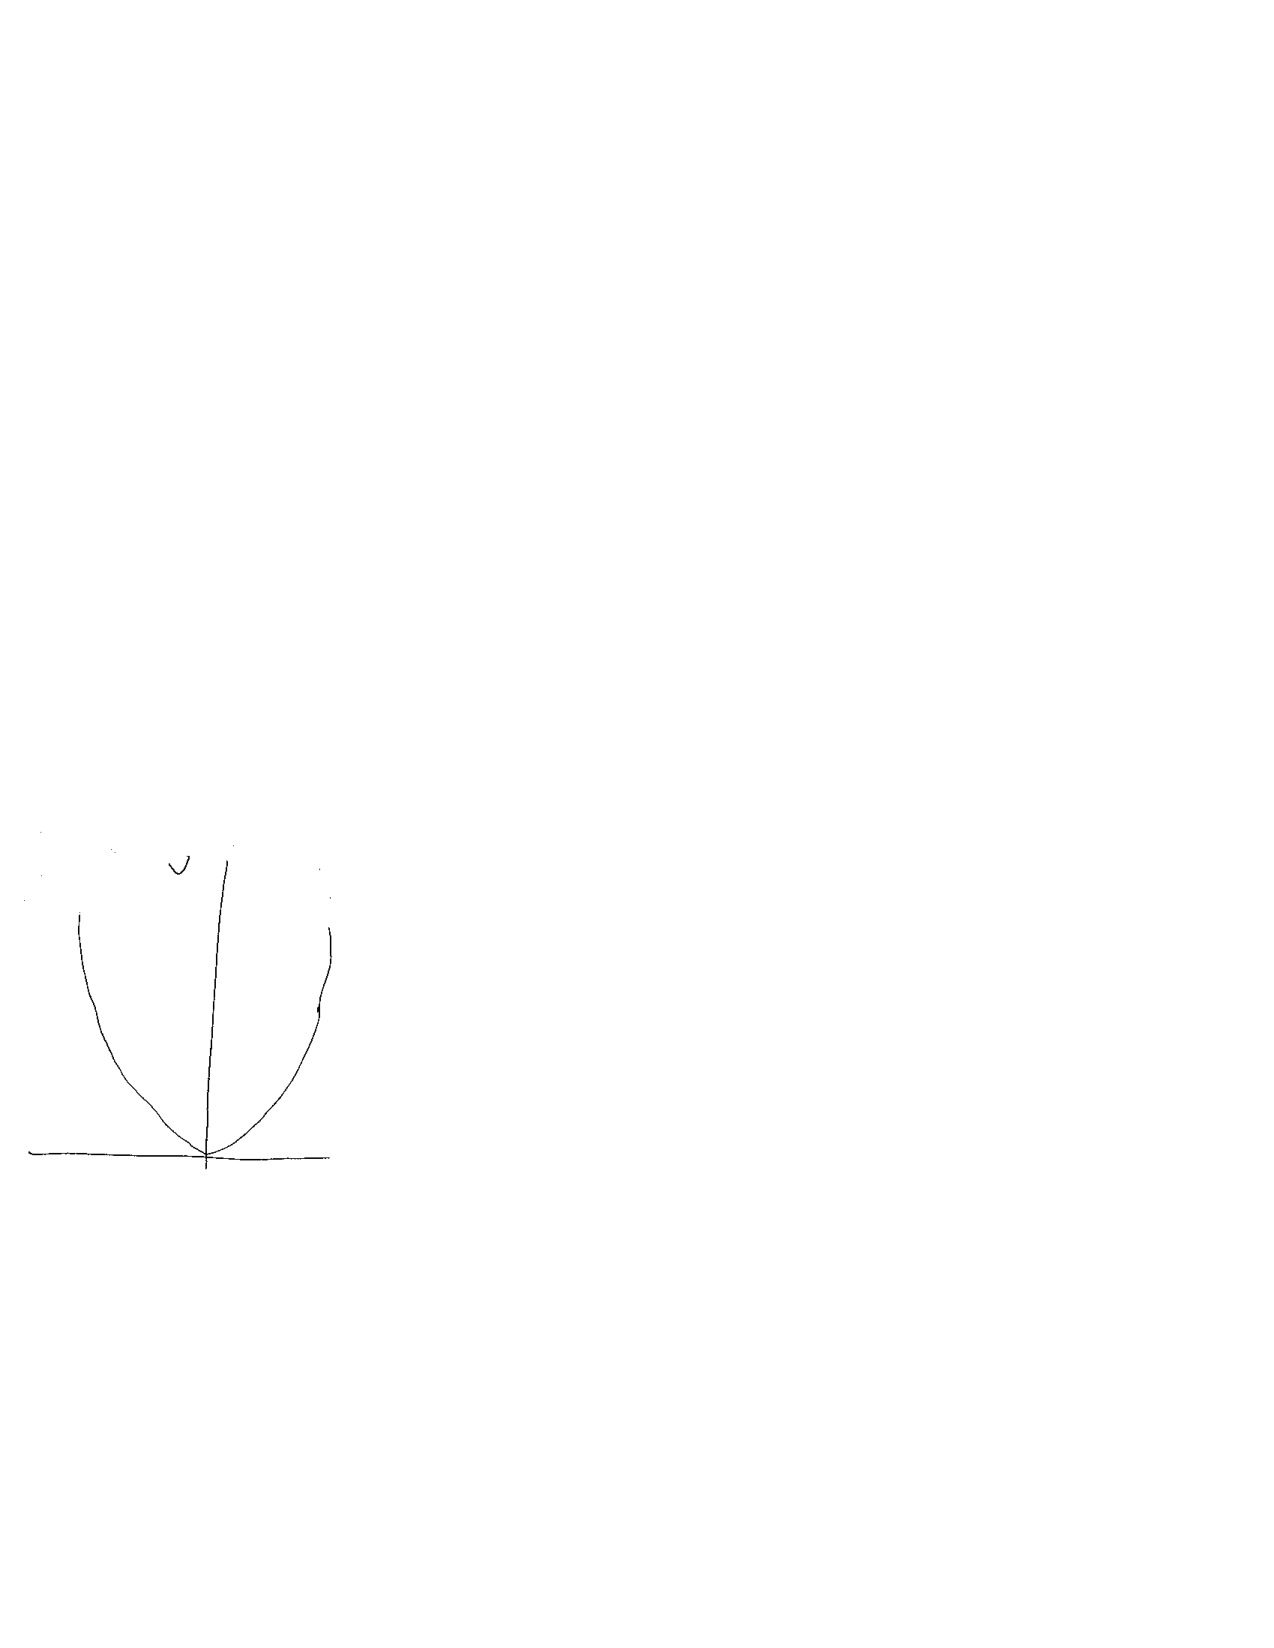
\includegraphics[width=0.3\textwidth]{./V_mu2positive.pdf}
\ec
the $\lambda \phi^4$ term leads to a direct four-point $\phi$ interaction.

\clearpage

\underline{Case b) $\mu^2 < 0$}\\

Now the L has a mass term with the wrong sign.  
(Relative ``+'' sign of the mass wrt to the kinetic term)

V now looks like:

\bc
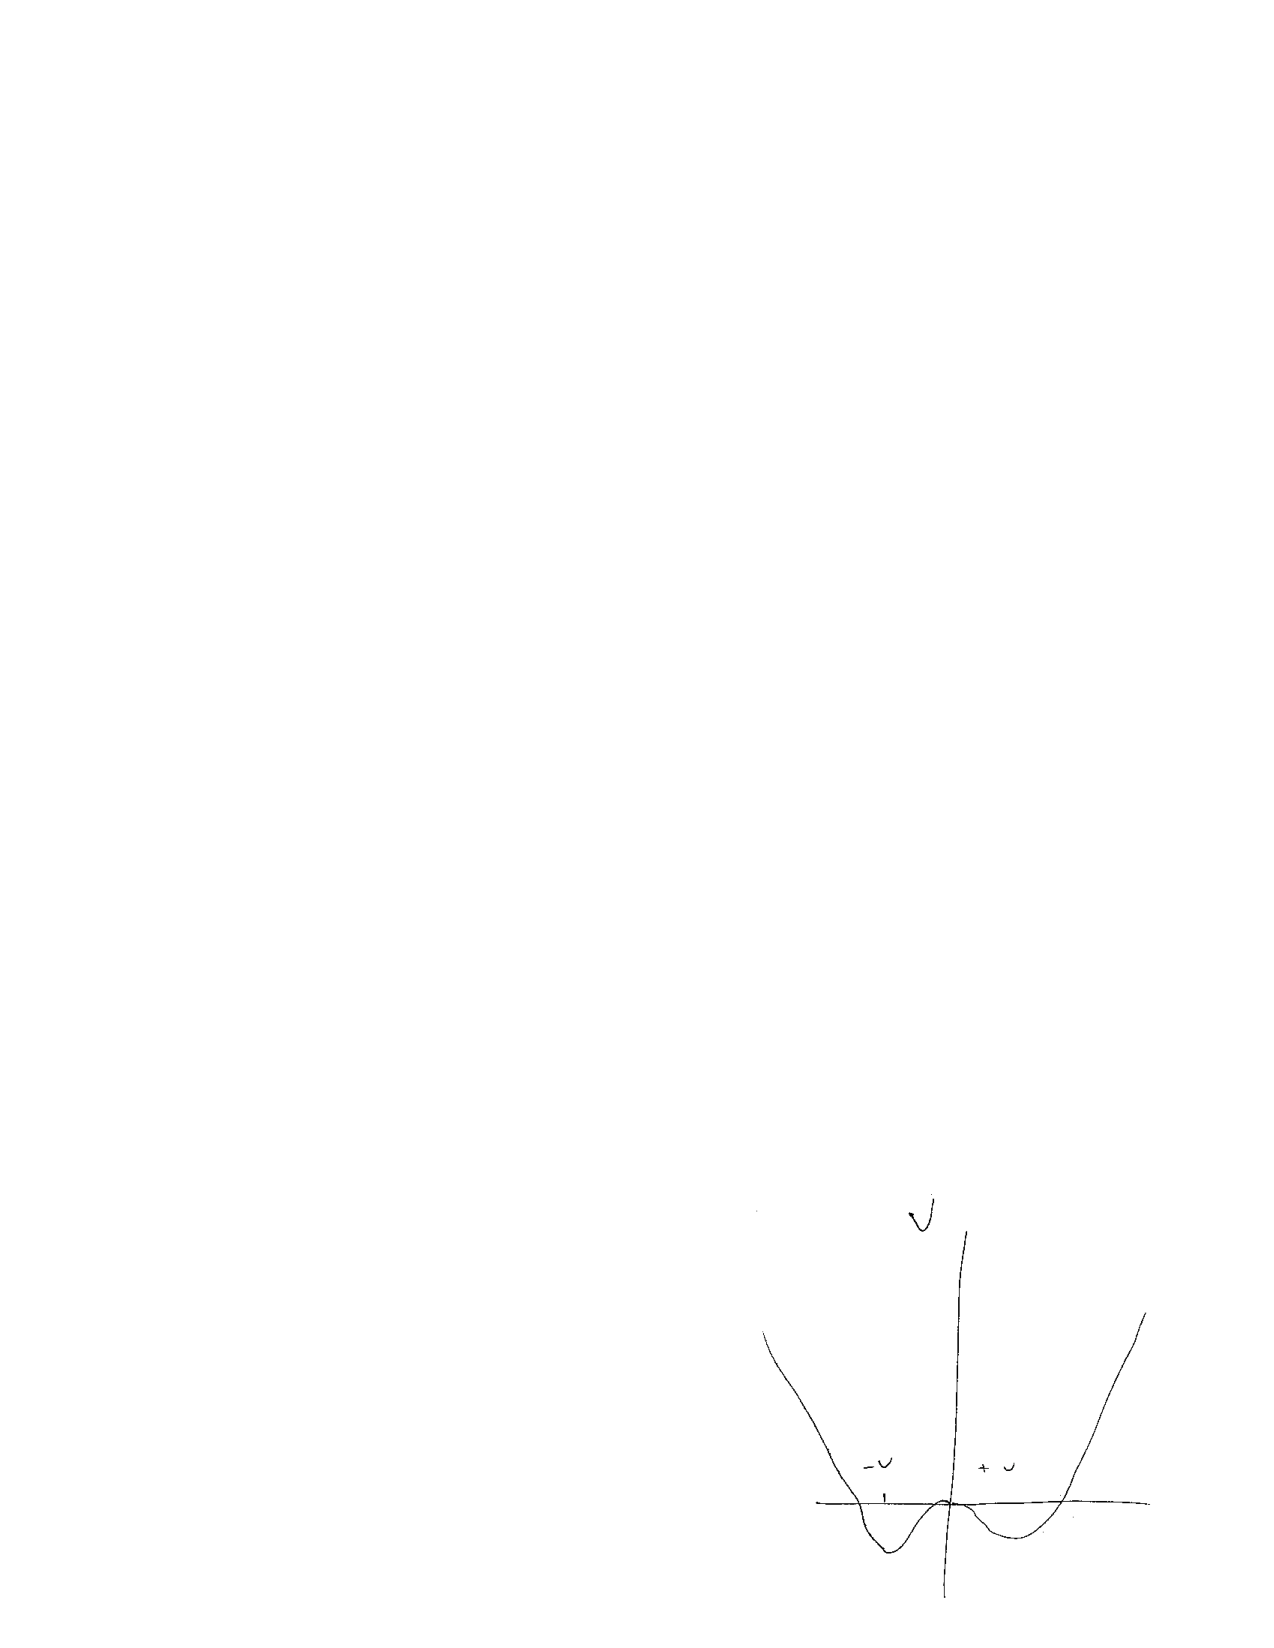
\includegraphics[width=0.4\textwidth]{./V_mu2negative.pdf}
\ec

Minimum at:
\be
\frac{\partial V}{\partial \phi} = \phi (\mu^2 + \lambda \phi^2) = 0 
\ee

\be
\phi = \pm v  \hspace*{1in} v = \sqrt{-\mu^2\lambda}
\ee

Now, $\phi=0$ does not correspond to a minimum.

Perturbative calculations should involve the expansion about minimum.  (either +v or -v) 

Take +v at random (``Spontaneously'') 

\be
\phi(x) = v + \eta(x)
\ee
where here $\eta(x)$ describes fluctuations about the minimum. 

Can then rewrite $L$ as 

\be
L' =  \frac{1}{2}(\partial \eta)^2 - \lambda v^2 \eta^2 - \lambda v \eta^3 - \frac{1}{2}\lambda \eta^4\ \rmt{+ constants}
\ee
Note that now the $\eta^2$ mass term has the correct sign with $m_\eta = \sqrt{-2\mu^2}$.

\begin{minipage}{0.5\textwidth}
Other terms give 3-point and 4-point\\
 $\eta$ interactions:
\end{minipage} \hfill
\begin{minipage}{0.5\textwidth}
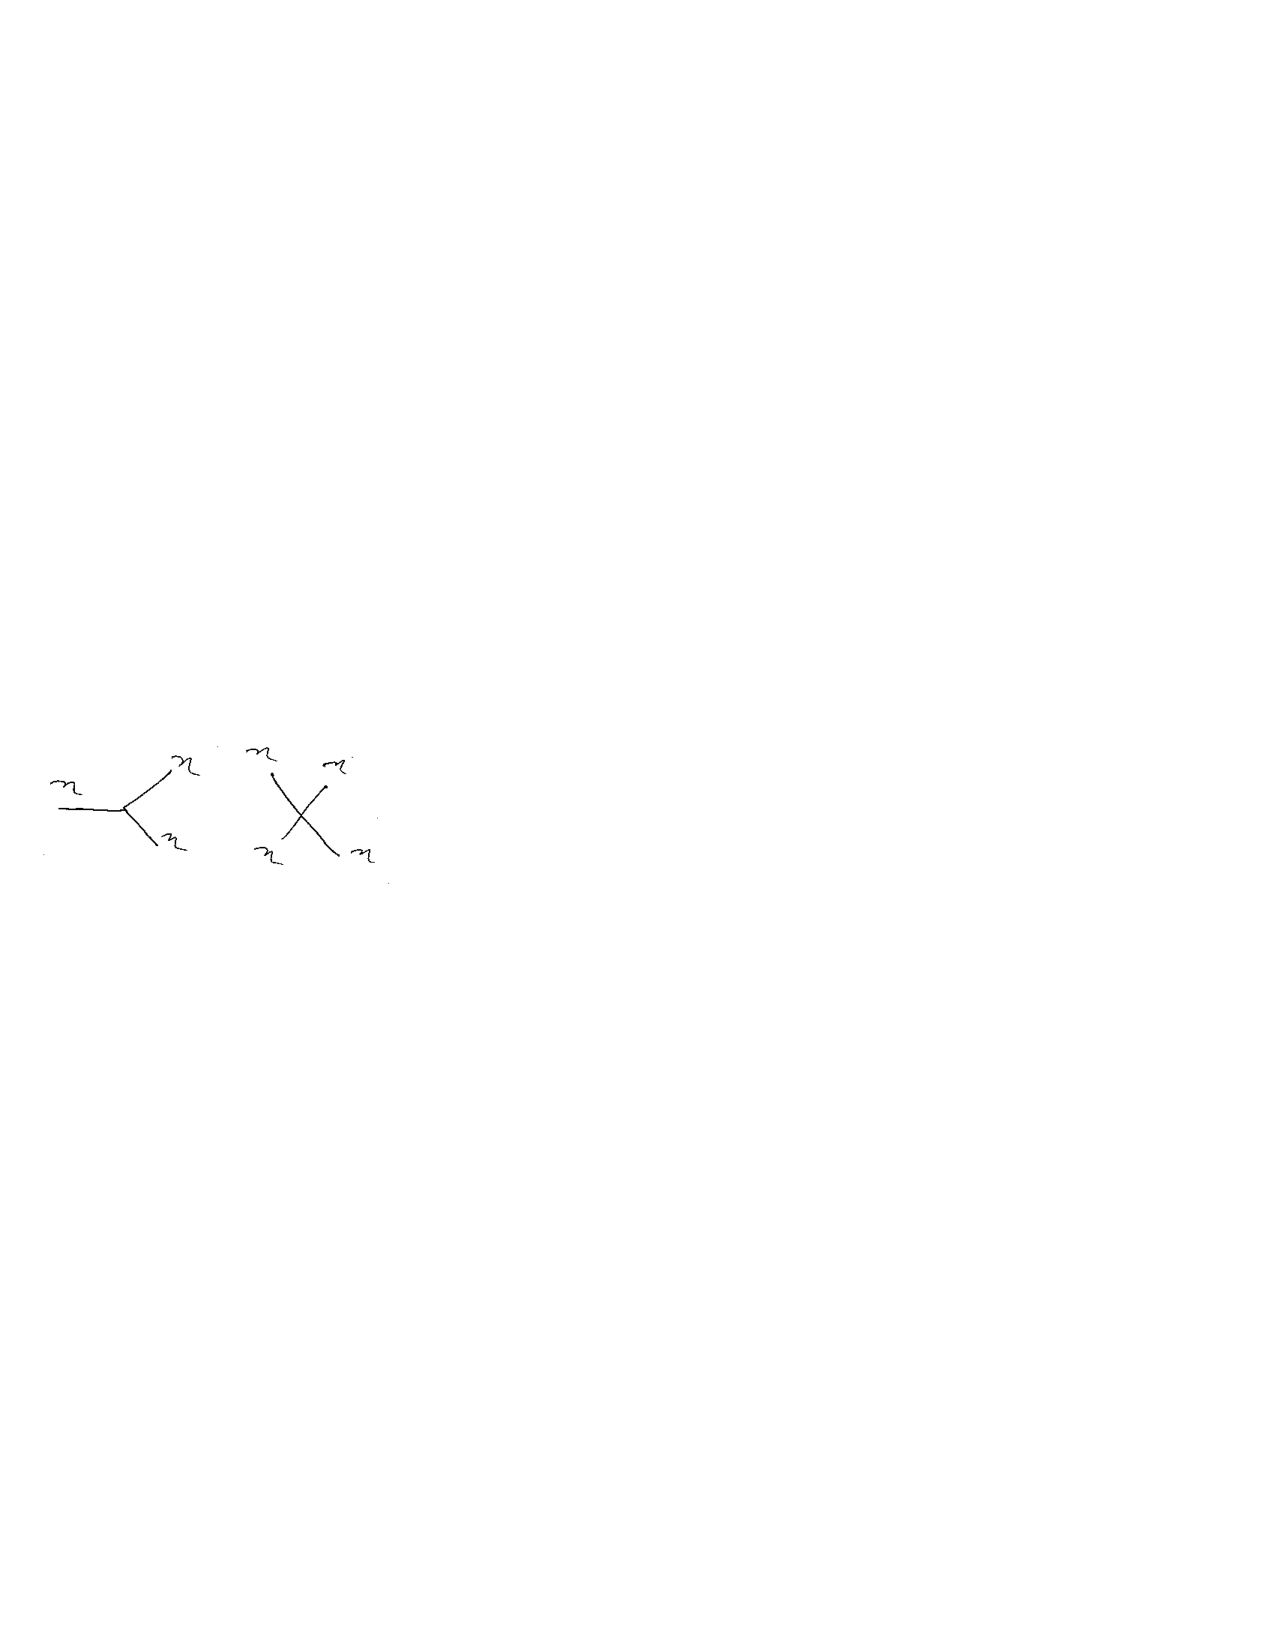
\includegraphics[width=1.0\textwidth]{./etaInteractions.pdf}
\end{minipage}

To summarize,
\bi
\item[-] Mass of $\eta$ was ``generated'' or ``revealed'' by ``Spontaneous Symmetry Breaking'' 
\item[-] The $\phi \rightarrow -\phi$ symmetry of $L$ is broken by the choice of the ground state.
\ei

This is an example that is seen in (very interesting) condensed matter systems. 

(eg: large ferromagnetic. 
Spins will align.  
All directions equally likely. 
Ground stat will be spins aligned in some direction
This ``choice'' of which way the spins point in the ground state breaks the rotational symmetry of the problem)


Superconductors and the buckling of a Needle are other examples of Spontaneous Symmetry Breaking.

\lineacross

\underline{Toy 2}  Repeat above with complex scalar field $\phi = \frac{1}{\sqrt{2}}\left(\phi_1 + i \phi_2\right)$

Will now consider the Lagrangian:
\be
L = \partial_\mu \phi^* \partial^\mu \phi - \mu^2 \phi^* \phi - \lambda(\phi^*\phi)^2
\ee
which is invariant under $\phi \rightarrow e^{i\alpha}\phi$  for arbitrary number  $\alpha$. (Global U(1) gauge symmetry.)

Now will take $\lambda > 0$ and $\mu^2 < 0$:

\be
L = \frac{1}{2}(\partial \phi_1)^2 + \frac{1}{2}(\partial \phi_2)^2 - \frac{1}{2}\mu^2(\phi_1^2 + \phi_2^2) - \frac{1}{4}\lambda(\phi_1^2 + \phi_2^2)^2
\ee

\begin{minipage}{0.5\textwidth}
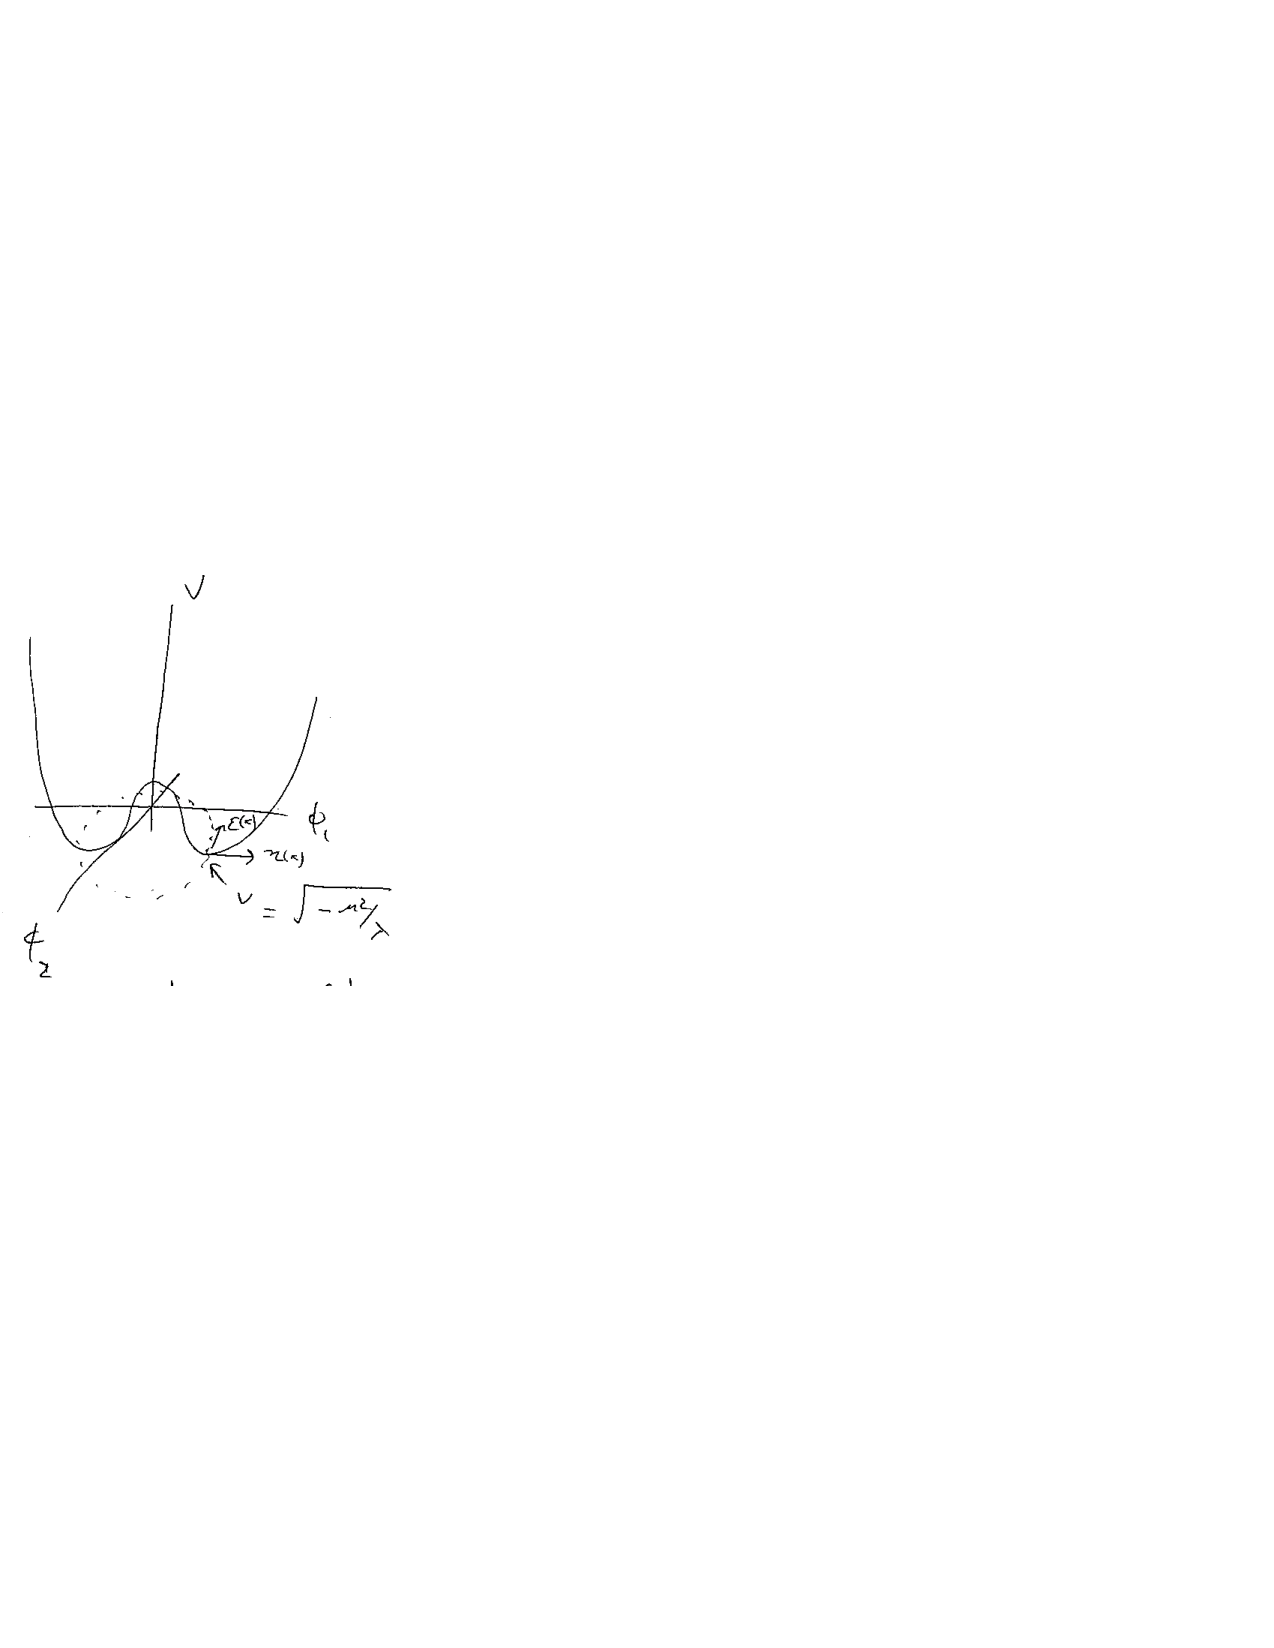
\includegraphics[width=1\textwidth]{./VComplex.pdf}
\end{minipage} \hfill
\begin{minipage}{0.5\textwidth}
Again, need to expand about min. \\
\underline{With out loss of generality} expand around $\phi_1 = v$ and $\phi_2 = 0$.\\
(like picking +v before) 
\be
\phi(x) = \sqrt{\frac{1}{2}}(v + \eta(x) + i\epsilon(x)
\ee
\end{minipage}

Now get a new Lagrangian
\be
L' = \frac{1}{2}(\partial \epsilon)^2 + \frac{1}{2}(\partial \eta)^2 + \mu^2\eta^2 + \mathcal{O}(\eta^3) + \mathcal{O}(\eta^4) + \mathcal{O}(\epsilon^3) + \mathcal{O}(\epsilon^4) 
\ee

with $\mu^2\eta^2 = -\frac{1}{2}m_\mu^2 \eta^2$ mass term for $\eta$ just as before.


However now have $\epsilon$ which is a \underline{mass-less} scalar ``Goldstone Boson''.

Problem, tried to give mass to a gauge boson and created a mass-less boson as well.

Intuitively, direction along $\epsilon$ is flat $\Rightarrow$ no resistance to excitations along that direction.   \underline{\underline{Crisis}}

Have not observed these massless gauge bosons. 

Lets try a local gauge theory (A miracle is about to happen...)

\clearpage

\lineacross

\underline{Higgs Mechanism} U(1) simplest example\\
(SM does this in $SU(2)_L$, getting closer...)

\be
\phi \rightarrow e^{i\alpha(x)} \phi  \hspace*{1in} \rmt{for arbitrary function $\alpha(x)$}
\ee

As for EM

\be
D_\mu = \partial_\mu - \underbrace{ieA_\mu}_{\rmt{gives coupling of $\phi$ to A}}
\ee

\be
A_\mu = A_\mu + \frac{1}{e}\partial_\mu \alpha(x)
\ee


\be
L = (D_\mu \phi)^*  (D^\mu \phi) - \mu^2 \phi^* \phi - \lambda(\phi^* \phi)^2 - \frac{1}{4}F_{\mu\nu}F^{\mu\nu}
\ee


(if $\mu^2 > 0$ QED w/massive charged scalar of mass $\mu$ and a 4-$\phi$ interaction term)

Now for $\mu^2 <0$, Again we do $\phi(x) \rightarrow \sqrt{\frac{1}{2}}(v + \eta(x) + i\epsilon(x)$

\be
L' = \frac{1}{2}(\partial \epsilon)^2 + \frac{1}{2}(\partial \eta)^2 - v^2\lambda\eta^2 + \frac{1}{2}e^2v^2A^2 - evA_\mu\partial^\mu\epsilon - \frac{1}{4}F_{\mu\nu}F^{\mu\nu} + \rmt{(interactions)}
\ee

\underline{3 particles} (Apparently...)

\bea
m_\epsilon &=& 0\ \rmt{(still problem)}\\
m_\eta &=& \sqrt{2\lambda v^2} \\
m_A &=& ev\ \rmt{dynamically generated mass for gauge feild}
\eea

This however cant be the spectrum because there are only 4 DoF before the expansion (2 scalar + 2 massless spin-1), but now seems like 5 = 2 (scalars) + 3 (massive spin-1).

So some of these apparent Dof are nonphysical\\
(Similar to picking a gauge in QED)

Try different expansion
\bea
\phi \rightarrow \frac{1}{\sqrt{2}}(v+h(x))e^{i\theta(x)/v}\\
A_\mu \rightarrow A_\mu + \frac{1}{ev} \partial \theta
\eea
this is a particular choice of gauge that give h-real.

\be
L'' = \frac{1}{2}(\partial h)^2  - \lambda v^2 h^2 + \frac{1}{2}e^2v^2A^2 - \lambda v h^3 - \frac{1}{4} \lambda h^4 + \frac{1}{2}e^2A^2 h^2  + v e^2 A^2h - \frac{1}{4} F^2
\ee
Now Goldstone boson does not appear in the theory! 

The apparent extra DoF was spurious
(only corresponds to a gauge transformation)

\underline{\underline{Spectra}}  (Physical)

2 massive interacting particles 
\bi
\item[$A_\mu$] - 3 DoF massive Spin-1
\item[$h$] - 1 DoF massive Spin-0
\ei
h-''Higgs boson''


Massless Goldstone Boson ``eaten'' by the $A_\mu$ to become the extra DoF needed for the longitudinal polarization.  

This is called the ``Higgs Mechanism''.

}
\end{document}


